\newcommand{\code}[1]{\texttt{#1}}

\chapter{Implementieren des hexagonalen Schachs nach Glinski}
Für die Implementierung des hexagonalen Schachs wird die Bibliothek \textit{pygame} genutzt. Diese vereinfacht es Spiele zu programmieren. Die Bibliothek stellt Methoden zur Verfügung, welche Fenster erstellen und Objekte malen. So eine Bibliothek erleichtert die Arbeit und ermöglicht einen schnelleren Start mit dem eigentlichen Programm. \textit{pygame} wird als Grundbaustein der Spieleprogrammierung in Python genutzt.

\begin{figure}[H]
    \centering
    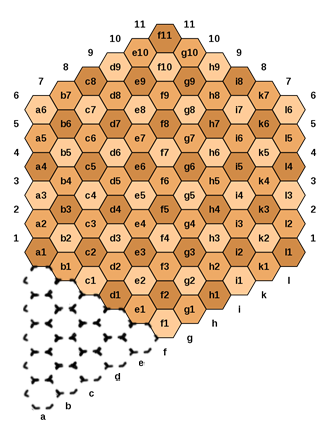
\includegraphics{images/hexIndex.png}
    \caption{Beschriftetes Spielfeld \protect\footnotemark}
    \label{fig:hex:index}
\end{figure}
\footnotetext{\url{https://commons.wikimedia.org/wiki/Category:Glinski\%27s_hexagonal_chess}}

Das Feld besteht aus 91 Hexagonen. Die Hexagone werden in einer zweidimensionalen Liste gespeichert. Mit dem ersten Index wird auf die Reihe, mit dem zweiten Index wird auf die Spalte zugegriffen. Mit den Indizes [0][0] wird das Feld  a6 angesprochen. Das nächste Feld in der Reihe ist bei b7 und wird mit den Indizes [0][1] angesprochen. Die Spalten a,b,c,d und e werden sobald sie kein Feld mehr enthalten mit \textit{None} aufgefüllt, damit die Formatierung der Felder bleibt.\par
Das Hexagon ist eine eigene Klasse. Die Klasse hat die Attribute Stein und Nachbarn. Die Nachbarn sind oben-links, oben, oben-rechts, unten-rechts, unten und unten-links vom Feld. Die Nachbarn sind Referenzen zu den Feldern. Dazu werden die Felder auch noch in einer Liste gespeichert, welche per Index sich in der genannten Reihenfolge aufrufen lassen. Die Nachbarn werden später für das Bewegen der Steine genutzt.\par
Ein Feld wird mit einer selbst geschriebenen Methode markiert. Das Feld wird markiert, wenn ein Feld als Bewegungsmöglichkeit gilt. Ein Feld gilt als mögliches Feld, wenn die Figur nach den Regeln von Glinski sich auf das Feld bewegen darf. Die Methode zum Markieren eines Feldes sieht wie folgt aus.

\begin{lstlisting}[language=python,caption={Felder markieren},captionpos=b,label={lst:hexa:markieren},numbers=left,frame=none,escapechar=|]
def mark_tile(self, tile):
  if not isinstance(tile, GameBoard.Hexagon):|\label{m:line2}|
    return None

  if tile.piece is not None:
    if tile.piece.white is self.white:
      return "taken"

    GameBoard.Hexagon(tile.screen, tile.outer_radius, tile.inner_radius,tile.x_pos, tile.y_pos, (255, 0, 0))|\label{m:line9}|
    tile.piece.move_towards(tile.x_pos, tile.y_pos, False, False)
    tile.is_destination = True
    return "enemy"
  
  GameBoard.Hexagon(tile.screen, tile.outer_radius, tile.inner_radius, tile.x_pos, tile.y_pos, (249, 215, 28))|\label{m:line14}|
  tile.is_destination = True
  return "field can be destination"
\end{lstlisting}

Die Methoden nimmt als Parameter ein Feld an. Wenn der Parameter kein Hexagon ist, was in Zeile \ref{m:line2} abgefragt wird, wird \textit{None} zurückgegeben. Mit \code{if tile.piece is not None:} wird überprüft ob auf dem Feld ein Stein steht. In der If-Abfrage wird weiter abgefragt, ob der Stein die gleiche Farbe hat wie die Figur, mit welcher gespielt wird. Ist das der Fall, wird „taken“ zurückgegeben. Ist auch das nicht der Fall, geht das Programm weiter und kommt zu dem Teil wo das Feld markiert wird. Zeile \ref{m:line9} erstellt ein rotes Hexagon auf der Position, wo das valide Feld liegt. Es muss ein neues Hexagon gemalt werden, da von dem alten nicht die Farbe geändert werden kann. Die Figur, die auf dem Feld stand, wird in diesem Prozess ebenfalls übermalt. Deswegen muss diese wieder in den Vordergrund bewegt werden. Das wird mit \code{tile.piece.move\_towards(tile.x\_pos, tile.y\_pos, False)} gemacht. Als letztes wird die Variable \textit{is\_destination} auf \textit{True} gesetzt. Diese Variable wird beim Klicken auf ein Feld abgefragt. Ist \textit{is\_destination True} wird der Stein auf das Feld bewegt, ist \textit{is\_destination False} passiert nichts. Am Ende des Rumpfes der If-Abfrage wird „enemy“ zurückgegeben. Nach der If-Abfrage folgen die Befehle, welche ausgeführt werden, wenn kein Stein auf dem Feld ist. Es wird ein gelbes, hexagonales Feld in Zeile \ref{m:line14} erstellt. Dadurch werden Felder mit Gegnern und freie Felder unterschieden. Ebenfalls wird die Variable \textit{is\_destination} auf \textit{True} gesetzt. Der Rückgabewert ist „field can be destination“.

\begin{lstlisting}[language=python,caption={Markierung aufheben},captionpos=b,label={lst:hexa:aufheben},numbers=left,frame=none,escapechar=|]
def tile_remove_mark(self, tile):
  if not isinstance(tile, GameBoard.Hexagon): |\label{yes,label}|
    return None

    GameBoard.Hexagon(tile.screen, tile.outer_radius, tile.inner_radius,tile.x_pos, tile.y_pos)
    if tile.piece is not None:
        tile.piece.move_towards(tile.x_pos, tile.y_pos, True, False)
        
    tile.is_destination = False
\end{lstlisting}

\textit{tile\_remove\_mark} entfernt die Markierung wieder. Damit keine Fehler auftreten wird in Zeile \ref{yes,label} erst geprüft, ob der Parameter \textit{tile} wirklich ein Hexagon ist. Danach malt Zeile \ref{r:line5} das Hexagon mit der Standartfarbe. Wenn auf dem Feld eine Figur war, wird diese wieder nach vorne bewegt. Als letztes wird \textit{is\_destination} wieder auf den Standartwert gesetzt.

Die Methode, welche die Figuren bewegt, ist ebenfalls eine eigene Methode. Jede Figur vererbt die Methode von der Elternklasse \textit{Piece}.

\begin{lstlisting}[language=python,caption={Figur bewegen},captionpos=b,label={lst:hexa:bewegen},numbers=left,frame=none,escapechar=|]
def move_towards(self, x, y, replace_bottom=True, moved=True):
    self.rect.x = x + self.offset[0]
    self.rect.y = y + self.offset[1]
    if replace_bottom:
        GameBoard.Hexagon(self.starting_tile.screen, self.starting_tile.outer_radius, self.starting_tile.inner_radius, self.starting_tile.x_pos, self.starting_tile.y_pos) 
        self.screen.blit(self.image, (self.rect.x, self.rect.y))
    pygame.display.flip()
    if moved:
        self.at_start = False

\end{lstlisting}

Die erwarteten Parameter sind die neuen X- und Y-Koordinaten, auf welchen die Figur gemalt wird. Die Standartparameter \textit{replace\_bottom} und \textit{moved} sind ohne Zuweisen beim Methodenaufruf jeweils \textit{False}. In den ersten beiden Zeilen der Methode werden die Koordinaten erneuert. Die Liste \textit{offset} ist ein statischer Wert, welcher die Figur auf das Feld zentriert. Beim Bewegen wird die alte Figur nicht entfernt. Der beste Weg die alte Figur zu entfernen, ist ein neues Hexagon über die alte Figur zu malen. \code{pygame.display.flip()} updatet das Fenster und die Änderungen werden angezeigt. Als letztes wird in der Methode die Variable \textit{at\_start} gleich \textit{False} gesetzt. \textit{at\_start} ist wichtig für die Steine, welche als erste Bewegungsmöglichkeiten besondere Regeln haben.\par
Die Figuren haben jeweils zwei Methoden, welche von der Elternklasse vererbt werden. Beim Klicken auf eine Figur wird die \textit{show\_moves} Methode aufgerufen. Jede Figur hat eine eigene \textit{show\_moves} Methode, welche alle Felder mithilfe der \textit{mark\_tile} Methode markiert.\par
Für die Figur werden die Seiten mit einer Schleife durchgelaufen. Als Beispiel wird der Turm genommen. Das Prinzip lässt sich auf die anderen Figuren übertragen. Bauern haben extra Regeln, welche sich aber aus dem Verhalten vom Turm ableiten lassen.

\begin{lstlisting}[language=python,caption={Figur zeige Bewegungsmöglichkeiten},captionpos=b,label={lst:hexa:show},numbers=left,frame=none,escapechar=|]
def show_moves(self):
    self.rows = [[], [], [], [], [], []]
    for i in range(len(self.starting_tile.sides)):
        tile = self.starting_tile.sides[i]
        while mark_tile(self, tile) is not None:
            self.rows[i].append(tile)
            if tile.piece is not None:
                break
            tile = tile.sides[i]

\end{lstlisting}

Mit der \textit{for}-Schleife werden die einzelnen Seiten durchgelaufen. Die Seite wird per Index bestimmt. Eine \textit{while}-Schleife läuft solange durch bis \textit{mark\_tile None} zurück gibt. Der Vorteil davon, ist dass das Feld direkt mit gefärbt wird. In der \textit{while}-Schleife werden die Felder an eine Liste angehängt. Beim Löschen der Markierung werden die Felder von der Liste durchgelaufen. Wenn die Schleife auf einen Spielstein trifft gibt \textit{mark\_tile} kein \textit{None} zurück. Deswegen muss die \textit{while}-Schleife unterbrochen werden, wenn auf einen Stein getroffen wird. Als letztes wird die Variable \textit{tile} zu dem passenden Nachbarn aktualisiert.\par
In dem \textit{main.py} werden die wechselnden Spielzüge verwaltet. Eine \textit{while}-Schleife läuft solange durch, bis das Fenster geschlossen wird oder ein König geschlagen wird. Ein Klick auf ein Feld wird wahrgenommen, indem die Distanz von jedem Feld zur Maus gemessen wird, sobald eine Taste gedrückt wird. Wenn die Distanz kleiner ist als ein \textit{treshhold} werden die möglichen Züge gezeigt. Wird ein valides Feld ausgewählt, bewegt sich die Figur zu dem Feld und der andere Spieler ist an der Reihe. Wenn ein Feld ausgewählt wird, was als nicht valide gilt, wird die Auswahl für die Figur aufgehoben und eine neue Figur kann ausgewählt werden.\par
Ein Problem bei der jetzigen Implementierung ist, dass Züge auch valide sind, wenn der König im Schach steht oder dadurch im Schach stehen würde. Durch die vielen Möglichkeiten, wie ein König im Schach stehen kann, wurde auf eine Implementierung des Features verzichtet und der Spieler muss jetzt selber auf seinen König aufpassen.
